\documentclass{tufte-book}
%\documentclass[twoside,symmetric]{tufte-book}
\hypersetup{colorlinks}% uncomment this line if you prefer colored hyperlinks (e.g., for onscreen viewing)

%%
% Book metadata
\title{Introduction \\to Python \thanks{Thanks to Edward R.~Tufte for his inspiration.}}
\author[The Tufte-LaTeX Developers]{CSEF}
\publisher{The Student Academy}

%%
% If they're installed, use Bergamo and Chantilly from www.fontsite.com.
% They're clones of Bembo and Gill Sans, respectively.
%\IfFileExists{bergamo.sty}{\usepackage[osf]{bergamo}}{}% Bembo
%\IfFileExists{chantill.sty}{\usepackage{chantill}}{}% Gill Sans

%\usepackage{microtype}

%%
% Just some sample text
\usepackage{lipsum}

%%
% For nicely typeset tabular material
\usepackage{booktabs}

%%
% For graphics / images
\usepackage{graphicx}
\setkeys{Gin}{width=\linewidth,totalheight=\textheight,keepaspectratio}
\graphicspath{{graphics/}}

%%
% Additional
\usepackage{units}
\usepackage{amsmath,amsfonts,amsthm} % Math packages
\usepackage{mathtools}% http://ctan.org/pkg/mathtools
%\usepackage{mparhack}
\usepackage{sectsty} % Allows customizing section commands
\usepackage[dvipsnames]{xcolor}
\usepackage{pgf,tikz}
\usepackage{pgfplots}
\usetikzlibrary{shapes,arrows}
\usetikzlibrary{patterns,fadings}
\usetikzlibrary{arrows}
 \usetikzlibrary{decorations.pathreplacing}
 \usetikzlibrary{snakes}
 \usetikzlibrary{spy}
 \usepackage{setspace}
% \usepackage{3dplot}
 \usepackage{cancel}
%\usepackage{physymb}
\usepackage{braket}
\usepackage{verbatim}
\usepackage{fancyvrb} % extended verbatim environments
\usepackage{framed}%To get shade behind text
\usepackage{pgfplots}
\usepackage{setspace}
\definecolor{shadecolor}{gray}{0.9}
%\usepackage[x11names]{xcolor}                     %Additional colors
%\usepackage{euler}  
\usepackage{framed}

%%%%%%%%%%%%%%%%%%%%%%%%%%%%%%%%%%%%%%%%%%%%%%%%%%%%%
% Default fixed font does not support bold face
\DeclareFixedFont{\ttb}{T1}{txtt}{bx}{n}{12} % for bold
\DeclareFixedFont{\ttm}{T1}{txtt}{m}{n}{12}  % for normal
% Custom colors
\usepackage{color}
\definecolor{normal}{rgb}{0,0.2,1}
\definecolor{lib}{rgb}{0.9,0.5,0}
\definecolor{str}{rgb}{0,0.7,0}
\definecolor{back}{rgb}{0.8,0.8,0.8}

\usepackage{listings}

% Python style for highlighting
\newcommand\pythonstyle{\lstset{
language=Python,
backgroundcolor=\color{back},
basicstyle=\ttm,
otherkeywords={*},             % Add keywords here
keywordstyle=\ttb\color{normal},
emph={__init__, in,from, import, and,not,or,as },          % Custom highlighting
emphstyle=\ttb\color{lib},    % Custom highlighting style
stringstyle=\color{str},
frame=single,
numbers=left,                         % Any extra options here
showstringspaces=false,
stepnumber=1,
commentstyle=\color{red}            % 
}}

% Python environment
\lstnewenvironment{python}[1][]
{
\pythonstyle
\lstset{#1}
}
{}

% Python for external files
\newcommand\pythonexternal[2][]{{
\pythonstyle
\lstinputlisting[#1]{#2}}}

% Python for inline
\newcommand\pythoninline[1]{{\pythonstyle\lstinline!#1!}}


%%%%%%%%%%%%%%%%%%%%%%%%%%%%%%%%%%%%%%%%%%%%%%%%%%%%%%%%%%


% The fancyvrb package lets us customize the formatting of verbatim
% environments.  We use a slightly smaller font.
\usepackage{fancyvrb}
\fvset{fontsize=\normalsize}

%%
% Prints argument within hanging parentheses (i.e., parentheses that take
% up no horizontal space).  Useful in tabular environments.
\newcommand{\hangp}[1]{\makebox[0pt][r]{(}#1\makebox[0pt][l]{)}}

%%
% Prints an asterisk that takes up no horizontal space.
% Useful in tabular environments.
\newcommand{\hangstar}{\makebox[0pt][l]{*}}

%%
% Prints a trailing space in a smart way.
\usepackage{xspace}




% Prints the month name (e.g., January) and the year (e.g., 2008)
\newcommand{\monthyear}{%
  \ifcase\month\or January\or February\or March\or April\or May\or June\or
  July\or August\or September\or October\or November\or
  December\fi\space\number\year
}


% Prints an epigraph and speaker in sans serif, all-caps type.
\newcommand{\openepigraph}[2]{%
  %\sffamily\fontsize{14}{16}\selectfont
  \begin{fullwidth}
  \sffamily\large
  \begin{doublespace}
  \noindent\allcaps{#1}\\% epigraph
  \noindent\allcaps{#2}% author
  \end{doublespace}
  \end{fullwidth}
}

% Inserts a blank page
\newcommand{\blankpage}{\newpage\hbox{}\thispagestyle{empty}\newpage}

\usepackage{units}

% Typesets the font size, leading, and measure in the form of 10/12x26 pc.
\newcommand{\measure}[3]{#1/#2$\times$\unit[#3]{pc}}

% Macros for typesetting the documentation
\newcommand{\hlred}[1]{\textcolor{Maroon}{#1}}% prints in red
\newcommand{\hangleft}[1]{\makebox[0pt][r]{#1}}
\newcommand{\hairsp}{\hspace{1pt}}% hair space
\newcommand{\hquad}{\hskip0.5em\relax}% half quad space
\newcommand{\TODO}{\textcolor{red}{\bf TODO!}\xspace}
\newcommand{\ie}{\textit{i.\hairsp{}e.}\xspace}
\newcommand{\eg}{\textit{e.\hairsp{}g.}\xspace}
\newcommand{\na}{\quad--}% used in tables for N/A cells
\providecommand{\XeLaTeX}{X\lower.5ex\hbox{\kern-0.15em\reflectbox{E}}\kern-0.1em\LaTeX}
\newcommand{\tXeLaTeX}{\XeLaTeX\index{XeLaTeX@\protect\XeLaTeX}}
% \index{\texttt{\textbackslash xyz}@\hangleft{\texttt{\textbackslash}}\texttt{xyz}}
\newcommand{\tuftebs}{\symbol{'134}}% a backslash in tt type in OT1/T1
\newcommand{\doccmdnoindex}[2][]{\texttt{\tuftebs#2}}% command name -- adds backslash automatically (and doesn't add cmd to the index)
\newcommand{\doccmddef}[2][]{%
  \hlred{\texttt{\tuftebs#2}}\label{cmd:#2}%
  \ifthenelse{\isempty{#1}}%
    {% add the command to the index
      \index{#2 command@\protect\hangleft{\texttt{\tuftebs}}\texttt{#2}}% command name
    }%
    {% add the command and package to the index
      \index{#2 command@\protect\hangleft{\texttt{\tuftebs}}\texttt{#2} (\texttt{#1} package)}% command name
      \index{#1 package@\texttt{#1} package}\index{packages!#1@\texttt{#1}}% package name
    }%
}% command name -- adds backslash automatically
\newcommand{\doccmd}[2][]{%
  \texttt{\tuftebs#2}%
  \ifthenelse{\isempty{#1}}%
    {% add the command to the index
      \index{#2 command@\protect\hangleft{\texttt{\tuftebs}}\texttt{#2}}% command name
    }%
    {% add the command and package to the index
      \index{#2 command@\protect\hangleft{\texttt{\tuftebs}}\texttt{#2} (\texttt{#1} package)}% command name
      \index{#1 package@\texttt{#1} package}\index{packages!#1@\texttt{#1}}% package name
    }%
}% command name -- adds backslash automatically
\newcommand{\docopt}[1]{\ensuremath{\langle}\textrm{\textit{#1}}\ensuremath{\rangle}}% optional command argument
\newcommand{\docarg}[1]{\textrm{\textit{#1}}}% (required) command argument
\newenvironment{docspec}{\begin{quotation}\ttfamily\parskip0pt\parindent0pt\ignorespaces}{\end{quotation}}% command specification environment
\newcommand{\docenv}[1]{\texttt{#1}\index{#1 environment@\texttt{#1} environment}\index{environments!#1@\texttt{#1}}}% environment name
\newcommand{\docenvdef}[1]{\hlred{\texttt{#1}}\label{env:#1}\index{#1 environment@\texttt{#1} environment}\index{environments!#1@\texttt{#1}}}% environment name
\newcommand{\docpkg}[1]{\texttt{#1}\index{#1 package@\texttt{#1} package}\index{packages!#1@\texttt{#1}}}% package name
\newcommand{\doccls}[1]{\texttt{#1}}% document class name
\newcommand{\docclsopt}[1]{\texttt{#1}\index{#1 class option@\texttt{#1} class option}\index{class options!#1@\texttt{#1}}}% document class option name
\newcommand{\docclsoptdef}[1]{\hlred{\texttt{#1}}\label{clsopt:#1}\index{#1 class option@\texttt{#1} class option}\index{class options!#1@\texttt{#1}}}% document class option name defined
\newcommand{\docmsg}[2]{\bigskip\begin{fullwidth}\noindent\ttfamily#1\end{fullwidth}\medskip\par\noindent#2}
\newcommand{\docfilehook}[2]{\texttt{#1}\index{file hooks!#2}\index{#1@\texttt{#1}}}
\newcommand{\doccounter}[1]{\texttt{#1}\index{#1 counter@\texttt{#1} counter}}

% Generates the index
\usepackage{makeidx}
\makeindex

\begin{document}

% Front matter
\frontmatter

% r.1 blank page
%\blankpage

% v.2 epigraphs
\newpage\thispagestyle{empty}

\openepigraph{%
The only shibboleth the West has is science. It is the premise of modernity and it defines itself as a rationality capable of, indeed requiring separation from politics, religion and really, society. Modernisation is to work towards this.
}{Bruno Latour}
\vfill
\openepigraph{%
The boundary between science fiction and social reality is an optical illusion.
}{Donna Haraway}


% r.3 full title page
\maketitle




% r.5 contents
\tableofcontents

\listoffigures

\listoftables

% r.7 dedication
\cleardoublepage
~\vfill
\begin{doublespace}
\noindent\fontsize{18}{22}\selectfont\itshape
\nohyphenation
The longest snake ever held captive is Medusa, a reticulated python (python reticulatus). On 12 October 2011, she was measured at 7.67 m long.% \mbox{Edward R.~Tufte} 
%and \mbox{Donald E.~Knuth}.
\end{doublespace}
\vfill
\vfill


% r.9 introduction
%\cleardoublepage
\chapter*{Note}

This physics text is an OpenSource academic project developed in abstraction at The Academy.  The manuscript is written in \LaTeX \ and makes use of the \doccls{tufte-book} and \doccls{tufte-handout} document classes.  

\vspace{2cm}

http://latex-project.org/ftp.html

https://git-scm.com/downloads

%%
% Start the main matter (normal chapters)
\mainmatter
<<<<<<< HEAD
\chapter{Libraries}
\section{Introduction}
Libraries in Python are extensions to the basic Pyhton coding. Python comes with some libraries of its own. But it is also possible to write your own libraries. But before you can use libraries you have to import the libraries that you want to use in your script. There are several ways how you can import libraries. Libraries are always imported at the beginning of a scrip.

\subsection{Importing Python Libraries}
The easiest way to import libraries is to use the import function. For these examples we will use the random library.
\marginnote{With this you have to put the libraries name in front of the function of the library}
\begin{python}
import random
print random.uniform(1,10)
\end{python}

If you want to rename a library before you are using it you can do the following
\begin{python}
import random as rndm
print rndm.uniform(1,10)
\end{python}

If you dont want to have to write a library name in front of it at all you can do
\begin{python}
from random import *
print uniform(1,10)
\end{python}

There is one other option how you can import libraries. If you use all of what we learned before we can use the following.
\marginnote{With this you can import a single function of a libary and you name the function.}
\begin{python}
from random import uniform as makeRandom
print makeRandom(1,10)
\end{python}

\subsection{Importing custom libraries}
If you want to use libraries you or someone else has written in python you can do that also. First you have to make sure that the script you want to import is in the same folder as the scripit you want to import it into. Lets asume we have to following script we want to use as a libary.
\begin{python}
def Bla():
    print "Bla"

def MyFunction(A)
    print A+A
\end{python}
Lets assume the scripts name is lib. Now if we want to use this in our main script we can do eaither of our ways. Use the file name as the libraries name.
\begin{python}
import lib
import lib as mylib
from lib import Bla as Tell
\end{python}
=======

<<<<<<< HEAD
>>>>>>> refs/remotes/Trismeg/master
%\include{introduction}
\

%\section{\textbf{For Loops, Nested For Loops}}
For in loop has the ability to iterate over the items of any sequence, such as a list or a string.

If a sequence contains an expression list, it is evaluated first. Then, the first item in the sequence is assigned to the iterating variable iterating var. Next, the statements block is executed. Each item in the list is assigned to iterating var, and the statement(s) block is executed until the entire sequence is exhausted.
\end{abstract}

\normalsize

\section{\textbf{PYTHON CODE}}

\section{\textbf{Syntax:}}
\begin{verbatim}
for var in sequence:
   statements
\end{verbatim}
   
\section{\textbf{example #1:}}   
\marginnote[40pt]{The goal is to print all the elements in the array}
\begin{shaded}
\begin{verbatim}
for i in ["hello", "hey", "yo"]:
    print i
\end{verbatim}
\end{shaded}

\section{\textbf{Output #1:}}
\begin{shaded}
\begin{verbatim}
>>> Hello
    hey
    yo
\end{verbatim}
\end{shaded}

\section{\textbf{example #2:}}   
\marginnote[40pt]{The goal is to print all the number in range 5. Note, that Python starts counting from 0}
\begin{shaded}
\begin{verbatim}
for i in range(5):
    print i
\end{verbatim}
\end{shaded}
    
\section{\textbf{Output #2:}}
\begin{shaded}
\begin{verbatim}
>>> 1
    2
    3
    4
    5
\end{verbatim}
\end{shaded}

\vspace{2cm}

\section{\textbf{NESTED FOR LOOPS}}
\begin{verbatim}
Python programming language allows to use one loop inside 
another loop. Following section shows few examples to illustrate
the concept.
\end{verbatim}


\section{\textbf{Syntax:}}
\begin{verbatim}
for iterating_var in sequence:
   for iterating_var in sequence:
      statements(s)
   statements(s)
\end{verbatim}

\section{\textbf{example #1:}}   
\marginnote[40pt]{The goal is to print every number from 0 to 5 three times in a row.}
\begin{shaded}
\begin{verbatim}
for i in range(5): #loop everything indented 5 times
    for j in range(3): #loop everything indented 3 times
        print i #print output of i

\end{verbatim}
\end{shaded}

\vspace{3cm}
\section{\textbf{Output 1:}}
\begin{shaded}
\begin{verbatim}
>>> 0
    0
    0
    1
    1
    1
    2
    2
    2
    3
    3
    3
    4
    4
    4
\end{verbatim}
\end{shaded}

\vspace{1cm}

\section{\textbf{example #2:}}   
\marginnote[40pt]{The goal is to create a 2D arrays that would be fulfilled with values of "1" or "0" depending on which number was randomly chosen by the computer}

\scriptsize
\begin{shaded}
\begin{verbatim}

import random #importing "random" library that will take random numbers for our program
x = [] #creating initial, empty array that will be fulfilled with other arrays later
for i in range(5): #loop everything indented 5 times
    r=[] #creates 5 more arrays
    for j in range(5): #loop everything indented 5 times
        if random.uniform(0,10)<3: #compare if randomly chosen number is smaller than 3
            r=r+[1] #if it is, add value of "1" inside the secondary array - r
        else: #or
            r=r+[0] #if it is bigger, add value of "0" inside the secondary array - r
    x.append(r) #add all of these secondary arrays to our main - x array. 
    #Basically we create 2D array.
print x #print our 2D array to see the output.

\end{verbatim}
\end{shaded}

\normalsize
\section{\textbf{Output 2:}}
\marginnote[40pt]{However, the numbers that you see here isn't the only output you can get. We used random uniforms and each time it will give different values.}
\begin{shaded}
\begin{verbatim}
>>> [[0, 0, 0, 1, 1], [1, 0, 0, 0, 0], [0, 0, 0, 0, 0],
    [0, 1, 0, 0, 0], [0, 0, 0, 0, 0]]
\end{verbatim}
\end{shaded}
   
=======

%ints and floats
%\chapter{Boolean}

\section{Intro}

boolean boolean

\section{Boolean Operators}

\section{Boolean Arithmetic}
<<<<<<< HEAD
\chapter{Array 1-D, 2-D, 3-D}
\section{Intro}
	Array is like a storage, it can fill with string or integer. In 1-D, 2-D it can also represents the x-axis and y axis.
\section{Creating arrays}
	Arrays is created buy blanket.\\ \ \\
\noindent Example:\\
\begin{verbatim}
	a=[ ]        *a is the array name that you want.
\end{verbatim}
The things in the [ ] and be store and when you want to access it you will need its position in the array and type like  a[0]\\ \ \\
\noindent Example:\\
\begin{verbatim}
	a=["apple","orange","banana"]
\end{verbatim}
If you want to print banana form the array, you may want to type\\
\begin{verbatim}
print a[2] 
\end{verbatim}
\section{Filling arrays}
	Everything can be store in the array, strings, integers, arrays. When you create an array you can fill things in it as the default  things that the array have.\\ \ \\
\noindent Example:
\begin{verbatim}
    a=["Billy","Bud",90,60,50]
    b=["Anne","Chow",90,95,100]
    c=["Jen","Bo",60,80,90]
\end{verbatim}

If you want to add things into the array that u create already, you can use \\ \ \\

\begin{verbatim}
     array_name=array_name+[Things you want to add]
\end{verbatim}

\noindent Example:\\ \ \\

\begin{verbatim}	
    a=[apple]
\end{verbatim}

\noindent and now I want to add orange into it, so we add\\ \ \\

\begin{verbatim}
    a=a+[orange]
\end{verbatim}	

\noindent To create 2-D or more array we need to create array in the nested for-loop.\\ \ \\
\noindent Example:
\begin{verbatim}
a=[]
for i in range(N):	*N how long you want the array to be
    b=[]    *This is a temporary array to generate every array inside the main array.
    for j in range(N):
        *Things you want to put in the array by b=b+[ ]
    a=a+[b]	    *Here put the temporary array back to the main array.
\end{verbatim}		


\section{Traversing array}
Traversing array is visiting each element in the array and do something. In 1-D we can do it with for loop to identify things in array.
Example:

\begin{verbatim}
a=[1,2,3]
for i in range(len(a))    *len(a) =  Numbers of elements in the array
    *Things put here can edit the specific element a[i]
\end{verbatim}
	
\noindent In 2-D we start using nested for-loop to identify the x-axis and y-axis. So we use nested for-loop to traversing it too.\\ \ \\
\noindent Example:
\begin{verbatim}
a=[[0,1],[0,0],[0,1]]
for i in range(len(a)):
    for j in range(len(a)):
        *Things put here can edit the specific element a[i][j]
\end{verbatim}
			
\noindent In 3-D we use more for-loop to identify the more dimension.\\ \ \\
\noindent Example:
\begin{verbatim}
a=[[[0,0],[0,0]],[[0,0],[0,0]]]
for x in range(len(a)):
    for y in range(len(a)):
        for z in range(len(a)):
            *Things put here can edit the specific element a[x][y][z]
\end{verbatim}
	
	
	
	
	
	

=======
>>>>>>> upstream/master
>>>>>>> upstream/master
%\include{rotational_kinematics}
%\include{forces}
%\include{work} 
%\include{momentum} 
	\begin{marginfigure}%
		\includegraphics[width=\linewidth]{lat.png}
		\caption{This is the logo of latex.}
		\label{fig:marginfig}
	\end{marginfigure}
	
	
	\normalsize
	
	%this generates 1cm of vertical space
	\vspace{1cm}
	\section{what is latex}
	
	LaTeX is a document preparation system for high-quality typesetting. It is most often used for medium-to-large technical or scientific documents but it can be used for almost any form of publishing.(Basically its a high-tech version of a pdf document maker that can do much more stuff than normal word documents.)

	

	
	\vspace{1cm}
	
	\section{this is how you start a latex file.}
	
	\marginnote[40pt]{Here you start you file by telling what kind of file you are making and the title and author of it. And begin the document.}
	\marginnote[40pt]{ And begin the document. remenber to have enddocument at the end of the paper.}

	\begin{framed}
		\begin{verbatim}
		\documentclass{tufte-handout}
		
		\title{Latex}
		
		\author[The Academy]{Tony/Zekang Lin}
		
		\begin{document}
		\end{verbatim}
	\end{framed}
		\section{this is some useful things you can do in latex file.}
		
		\marginnote[40pt]{you can use margin figure or figure to include pictures as a note or just something that you want to show.it will auto matically lable the picture as figure + the number of the image.}
		\marginnote[40pt]{use marginnote to add notes.}
		\marginnote[40pt]{shaded can help you shade what you are going to write and verbatim will allow you to write your codes in latex.}
		
		\begin{framed}
			\begin{verbatim}
\begin{marginfigure}%
\includegraphics[width=\linewidth]{XXXXX.png}
\caption{This is the logo of latex.}
\label{fig:marginfig}
\end{marginfigure}


\marginnote[30pt]{DXXXXXXXXXXXXXXXXXXXXXXXXXXXXX}


\begin{shaded}
\begin{verbatim}
			\end{verbatim}
		\end{framed}
		
\vspace{1cm}
\section{why do we use latex.}
	\begin{verbatim}
Latex is easy to use and there are many stuff that latex will 
automaticallydo for you, such as it will automatically write 
the date that you last edited and autometically lable the number 
of images you added to the paper.
	\end{verbatim}
	
	\vspace{1cm}
	\section{this is what a Latex paper can look like:}
	\marginnote[40pt]{}
		\begin{figure}
			\includegraphics[width=\linewidth]{latresult.png}
			\caption{this is what latex paper can look like.}
			\label{fig:marginfig}
		\end{figure}
	
 
\definecolor{shadecolor}{rgb}{0.9,0.9,0.9}











\chapter{While Loops}

A {\color{red}while loop} statement in Python programming language repeatedly executes a target statement as long as a given condition is true.

\vspace{1cm}
The condition may be any expression, and true is any non-zero value. The loop iterates while the condition is true.When the condition becomes false, program control passes to the line immediately following the loop.In Python, all the statements indented by the same number of character spaces after a programming construct are considered to be part of a single block of code. Python uses indentation as its method of grouping statements.

\begin{marginfigure}
  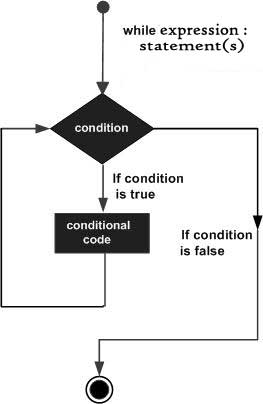
\includegraphics[width=\linewidth]{whileloop.jpeg}
  \caption{Flow diagram about how the while loop works}
  \label{fig:marginfig}
\end{marginfigure}

\vspace{0.5cm}
\subsection{Python code example}
\begin{framed}
\begin{verbatim}

count = 0
while (count < 9):
   print 'The count is:', count
   count = count + 1

print "Good bye!"

\end{verbatim}
\end{framed}

\subsection{Output}
\marginnote[40pt]{The code will produce the following output.}
\begin{shaded}
\begin{verbatim}
>>> 
The count is: 0
The count is: 1
The count is: 2
The count is: 3
The count is: 4
The count is: 5
The count is: 6
The count is: 7
The count is: 8
Good bye!
>>> 
\end{verbatim}
\end{shaded}

\subsection{Infinite Loop}
A loop becomes {\color{red}infinite loop} if a condition never becomes {\textbf{FALSE}}. You must use caution when using while loops because of the possibility that this condition never resolves to a FALSE value. This results in a loop that never ends. Such a loop is called an infinite loop.

An infinite loop might be useful in client/server programming where the server needs to run continuously so that client programs can communicate with it as and when required.
\marginnote[40pt]{This python code is an example of how infinite loop can be created.}
\begin{framed}
\begin{verbatim}
var = 1
while var == 1:
   num = raw_input("Enter a number  :")
   print "You entered: ", num

print "Good bye!"
\end{verbatim}
\end{framed}

\marginnote[40pt]{This code creates an infinite loop where it will need your input of any number.Once you input any number, it will output it like if you input "X" it will show back "X".}
\begin{shaded}
\begin{verbatim}

Enter a number  :X
You entered:  x
Enter a number  :Y
You entered:  Y
Enter a number  :Z
You entered:  Z
Enter a number between :

\end{verbatim}
\end{shaded}

To break the loop you will either need to add the "{\color{red}break}" command in your code OR press {\textbf{CTRL+C} to exit the program.

\subsection{Using else statements with while loops}
Python supports to have an else statement associated with a loop statement.

If the {\color{red}else statement} is used with a while loop, the else statement is executed when the condition becomes false.

\vspace{1cm}







\begin{framed}
\begin{verbatim}

count = 0
while count < 5:
   print count, " is  less than 5"
   count = count + 1
else:
   print count, " is not less than 5"

\end{verbatim}
\end{framed}

\marginnote[-140pt]{The following code illustrates the combination of an else statement with a while statement that prints a number as long as it is less than 5, otherwise else statement gets executed.}

\marginnote[40pt]{This is the output in python when the code above is executed.}
\begin{shaded}
\begin{verbatim}
>>> 
0 is less than 5
1 is less than 5
2 is less than 5
3 is less than 5
4 is less than 5
5 is not less than 5
>>> 
\end{verbatim}
\end{shaded}










%\bibliography{sample-handout}
\bibliographystyle{plainnat}



\printindex

\end{document}


